\documentclass[11pt]{article}\usepackage[]{graphicx}\usepackage[]{color}
%% maxwidth is the original width if it is less than linewidth
%% otherwise use linewidth (to make sure the graphics do not exceed the margin)
\makeatletter
\def\maxwidth{ %
  \ifdim\Gin@nat@width>\linewidth
    \linewidth
  \else
    \Gin@nat@width
  \fi
}
\makeatother

\definecolor{fgcolor}{rgb}{0.345, 0.345, 0.345}
\newcommand{\hlnum}[1]{\textcolor[rgb]{0.686,0.059,0.569}{#1}}%
\newcommand{\hlstr}[1]{\textcolor[rgb]{0.192,0.494,0.8}{#1}}%
\newcommand{\hlcom}[1]{\textcolor[rgb]{0.678,0.584,0.686}{\textit{#1}}}%
\newcommand{\hlopt}[1]{\textcolor[rgb]{0,0,0}{#1}}%
\newcommand{\hlstd}[1]{\textcolor[rgb]{0.345,0.345,0.345}{#1}}%
\newcommand{\hlkwa}[1]{\textcolor[rgb]{0.161,0.373,0.58}{\textbf{#1}}}%
\newcommand{\hlkwb}[1]{\textcolor[rgb]{0.69,0.353,0.396}{#1}}%
\newcommand{\hlkwc}[1]{\textcolor[rgb]{0.333,0.667,0.333}{#1}}%
\newcommand{\hlkwd}[1]{\textcolor[rgb]{0.737,0.353,0.396}{\textbf{#1}}}%
\let\hlipl\hlkwb

\usepackage{framed}
\makeatletter
\newenvironment{kframe}{%
 \def\at@end@of@kframe{}%
 \ifinner\ifhmode%
  \def\at@end@of@kframe{\end{minipage}}%
  \begin{minipage}{\columnwidth}%
 \fi\fi%
 \def\FrameCommand##1{\hskip\@totalleftmargin \hskip-\fboxsep
 \colorbox{shadecolor}{##1}\hskip-\fboxsep
     % There is no \\@totalrightmargin, so:
     \hskip-\linewidth \hskip-\@totalleftmargin \hskip\columnwidth}%
 \MakeFramed {\advance\hsize-\width
   \@totalleftmargin\z@ \linewidth\hsize
   \@setminipage}}%
 {\par\unskip\endMakeFramed%
 \at@end@of@kframe}
\makeatother

\definecolor{shadecolor}{rgb}{.97, .97, .97}
\definecolor{messagecolor}{rgb}{0, 0, 0}
\definecolor{warningcolor}{rgb}{1, 0, 1}
\definecolor{errorcolor}{rgb}{1, 0, 0}
\newenvironment{knitrout}{}{} % an empty environment to be redefined in TeX

\usepackage{alltt}
%\usepackage[showframe]{geometry}
\usepackage[table]{xcolor}
\usepackage{caption}
\usepackage{lscape,verbatim,mathrsfs}
\usepackage{graphics,amsmath,pstricks}
\usepackage{amssymb,enumerate}
\usepackage{amsbsy,amsmath,amsthm,amsfonts, amssymb}
\usepackage{graphicx, rotate, array}
\usepackage{geometry,multirow}
\usepackage{color,soul}
\usepackage{float}
%\usepackage{hyperref}
\usepackage[authoryear,round]{natbib}
%\renewcommand{\baselinestretch}{1.9}
\usepackage{tcolorbox}
\renewcommand{\familydefault}{cmss}
\textwidth=6.65in \textheight=9.7in
\parskip=.025in
\parindent=0in
\oddsidemargin=-0.1in \evensidemargin=-.1in \headheight=-.6in
\footskip=0.5in \DeclareMathOperator*{\argmax}{argmax}
\DeclareMathOperator*{\argmin}{argmin}
\IfFileExists{upquote.sty}{\usepackage{upquote}}{}
\begin{document}







CONT




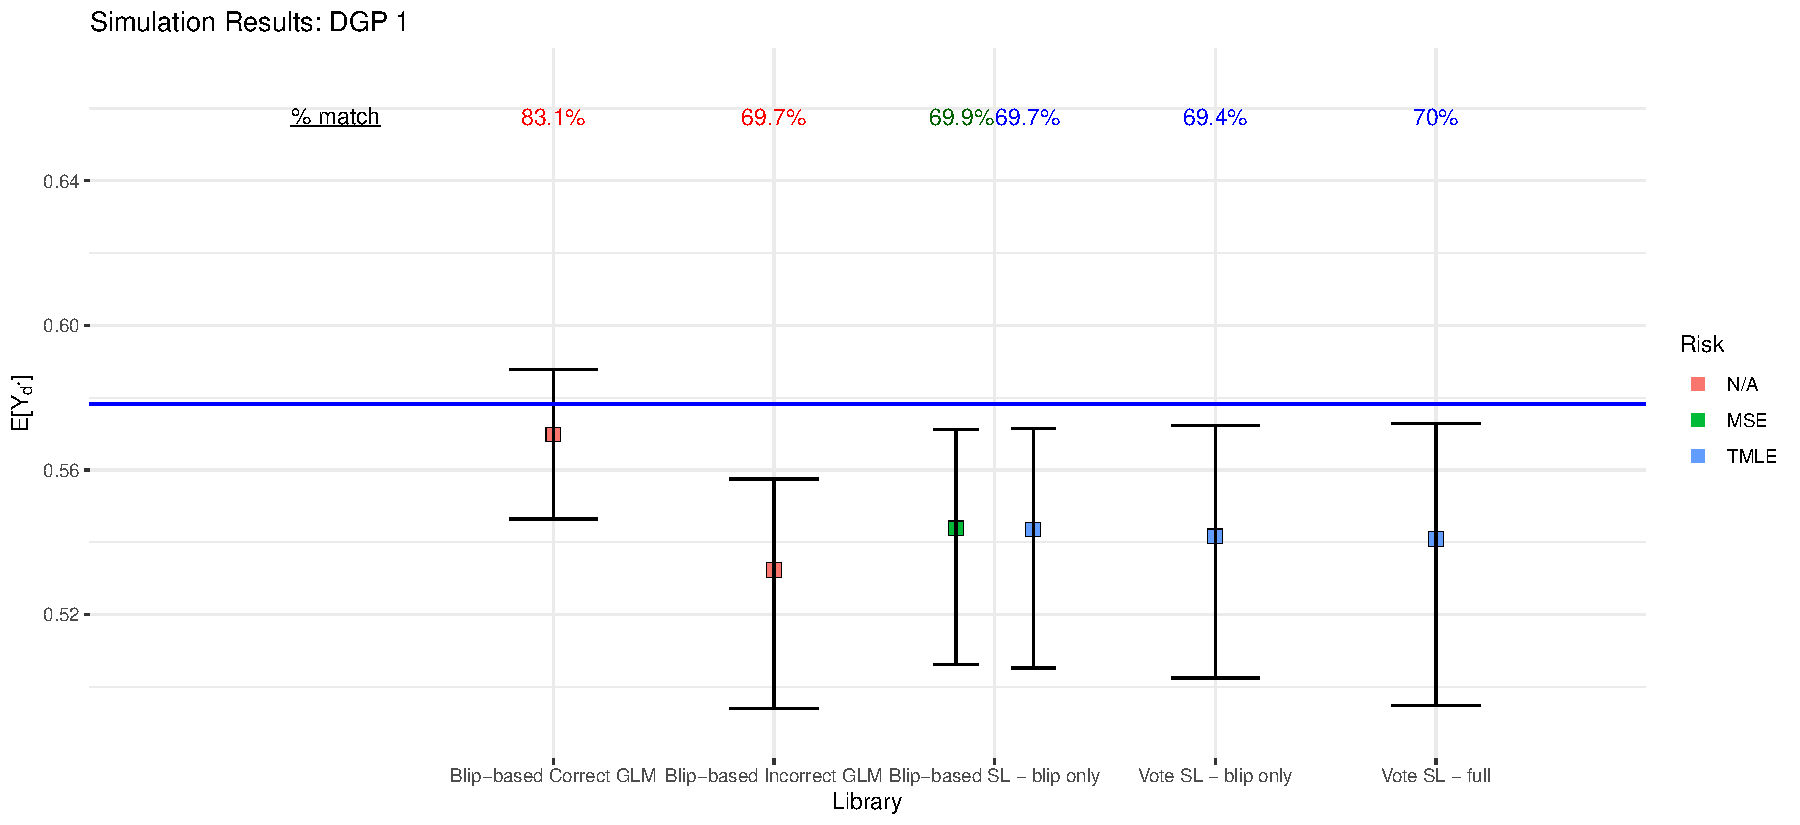
\includegraphics[width=\maxwidth]{figure/ODTR_DGP_cont_step1a-1} 


% latex table generated in R 3.5.1 by xtable 1.8-4 package
% Sat Sep 14 17:01:29 2019
\begin{table}[ht]
\centering
\scalebox{0.7}{
\begin{tabular}{rrr}
  \hline
 & MSE & TMLE \\ 
  \hline
Bias & -0.03435 & -0.03470 \\ 
  Variance & 0.00032 & 0.00029 \\ 
  MSE & 0.00150 & 0.00150 \\ 
  coef.SL.glm & 0.09546 & 0.12654 \\ 
  coef.SL.mean & 0.27211 & 0.14098 \\ 
  coef.SL.glm.interaction & 0.24739 & 0.18893 \\ 
  coef.SL.earth & 0.12259 & 0.15239 \\ 
  coef.SL.nnet & 0.07484 & 0.12411 \\ 
  coef.SL.svm & 0.09453 & 0.13560 \\ 
  coef.SL.rpart & 0.09307 & 0.13145 \\ 
   \hline
\end{tabular}
}
\caption{cont - 1a} 
\end{table}
% latex table generated in R 3.5.1 by xtable 1.8-4 package
% Sat Sep 14 17:01:29 2019
\begin{table}[ht]
\centering
\scalebox{0.7}{
\begin{tabular}{rr}
  \hline
 & TMLE \\ 
  \hline
Bias & -0.03724 \\ 
  Variance & 0.00041 \\ 
  MSE & 0.00179 \\ 
  coef.DonV.DonV.SL.glm\_All & 0.06519 \\ 
  coef.DonV.DonV.SL.mean\_All & 0.04298 \\ 
  coef.DonV.DonV.SL.glm.interaction\_All & 0.12039 \\ 
  coef.DonV.DonV.SL.earth\_All & 0.09553 \\ 
  coef.DonV.DonV.SL.nnet\_All & 0.07569 \\ 
  coef.DonV.DonV.SL.svm\_All & 0.11764 \\ 
  coef.DonV.DonV.SL.rpart\_All & 0.06990 \\ 
  coef.Qlearn & 0.05995 \\ 
  coef.OWL & 0.05416 \\ 
  coef.EARL & 0.04118 \\ 
  coef.optclass & 0.08226 \\ 
  coef.RWL & 0.04208 \\ 
  coef.treatall & 0.05255 \\ 
  coef.treatnone & 0.08051 \\ 
   \hline
\end{tabular}
}
\caption{cont - 1b} 
\end{table}
% latex table generated in R 3.5.1 by xtable 1.8-4 package
% Sat Sep 14 17:01:29 2019
\begin{table}[ht]
\centering
\scalebox{0.7}{
\begin{tabular}{rr}
  \hline
 & TMLE \\ 
  \hline
Bias & -0.03658 \\ 
  Variance & 0.00034 \\ 
  MSE & 0.00168 \\ 
  coef.DonV.DonV.SL.glm\_All & 0.11526 \\ 
  coef.DonV.DonV.SL.mean\_All & 0.12267 \\ 
  coef.DonV.DonV.SL.glm.interaction\_All & 0.17436 \\ 
  coef.DonV.DonV.SL.earth\_All & 0.14708 \\ 
  coef.DonV.DonV.SL.nnet\_All & 0.13212 \\ 
  coef.DonV.DonV.SL.svm\_All & 0.18544 \\ 
  coef.DonV.DonV.SL.rpart\_All & 0.12307 \\ 
   \hline
\end{tabular}
}
\caption{cont - 1c} 
\end{table}
% latex table generated in R 3.5.1 by xtable 1.8-4 package
% Sat Sep 14 17:01:29 2019
\begin{table}[ht]
\centering
\scalebox{0.7}{
\begin{tabular}{rrr}
  \hline
 & MSE & TMLE \\ 
  \hline
Bias & -0.00842 & -0.00842 \\ 
  Variance & 0.00012 & 0.00012 \\ 
  MSE & 0.00019 & 0.00019 \\ 
  estimates..1.....grep.colnames.estimates..1.....pattern....coef... & 1.00000 & 1.00000 \\ 
   \hline
\end{tabular}
}
\caption{cont - step3a} 
\end{table}
% latex table generated in R 3.5.1 by xtable 1.8-4 package
% Sat Sep 14 17:01:29 2019
\begin{table}[ht]
\centering
\scalebox{0.7}{
\begin{tabular}{rrr}
  \hline
 & MSE & TMLE \\ 
  \hline
Bias & -0.04580 & -0.04580 \\ 
  Variance & 0.00027 & 0.00027 \\ 
  MSE & 0.00237 & 0.00237 \\ 
  estimates..1.....grep.colnames.estimates..1.....pattern....coef... & 1.00000 & 1.00000 \\ 
   \hline
\end{tabular}
}
\caption{cont - step5a} 
\end{table}




























BIN




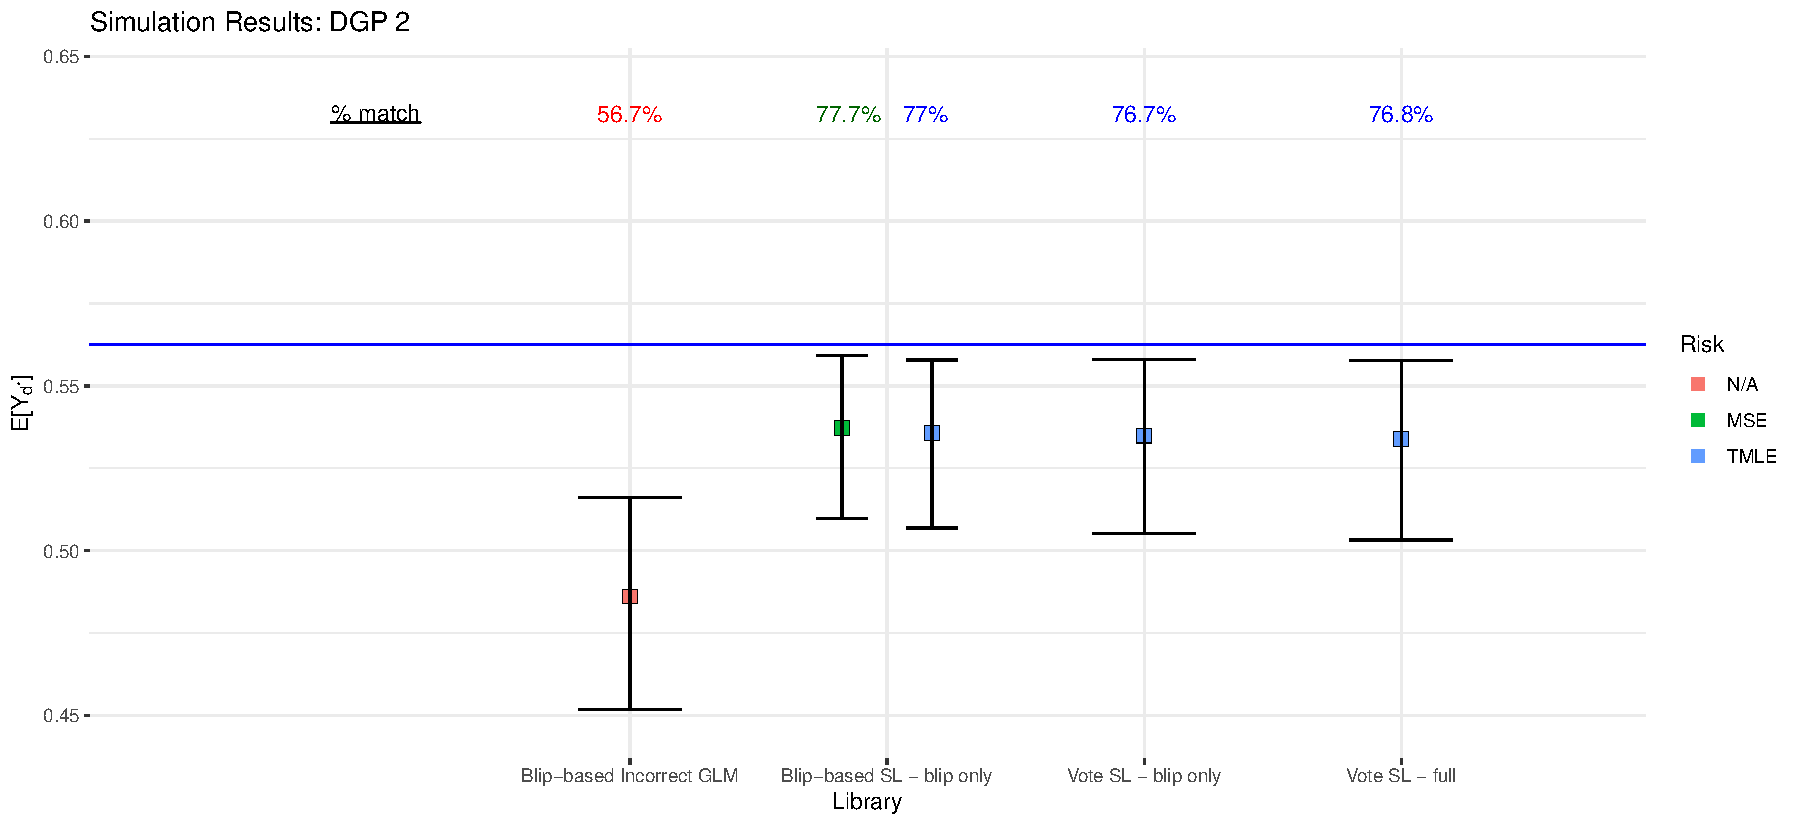
\includegraphics[width=\maxwidth]{figure/ODTR_DGP_bin_step1a-1} 


% latex table generated in R 3.5.1 by xtable 1.8-4 package
% Sat Sep 14 17:01:30 2019
\begin{table}[ht]
\centering
\scalebox{0.7}{
\begin{tabular}{rrr}
  \hline
 & MSE & TMLE \\ 
  \hline
Bias & -0.02533 & -0.02683 \\ 
  Variance & 0.00015 & 0.00016 \\ 
  MSE & 0.00080 & 0.00088 \\ 
  coef.SL.glm & 0.05282 & 0.09355 \\ 
  coef.SL.mean & 0.13224 & 0.11436 \\ 
  coef.SL.glm.interaction & 0.03420 & 0.07687 \\ 
  coef.SL.earth & 0.27292 & 0.26934 \\ 
  coef.SL.nnet & 0.10743 & 0.09954 \\ 
  coef.SL.svm & 0.19965 & 0.17341 \\ 
  coef.SL.rpart & 0.20075 & 0.17293 \\ 
   \hline
\end{tabular}
}
\caption{bin - 1a} 
\end{table}
% latex table generated in R 3.5.1 by xtable 1.8-4 package
% Sat Sep 14 17:01:30 2019
\begin{table}[ht]
\centering
\scalebox{0.7}{
\begin{tabular}{rr}
  \hline
 & TMLE \\ 
  \hline
Bias & -0.02876 \\ 
  Variance & 0.00020 \\ 
  MSE & 0.00103 \\ 
  coef.DonV.DonV.SL.glm\_All & 0.03969 \\ 
  coef.DonV.DonV.SL.mean\_All & 0.04205 \\ 
  coef.DonV.DonV.SL.glm.interaction\_All & 0.03846 \\ 
  coef.DonV.DonV.SL.earth\_All & 0.17439 \\ 
  coef.DonV.DonV.SL.nnet\_All & 0.06079 \\ 
  coef.DonV.DonV.SL.svm\_All & 0.09472 \\ 
  coef.DonV.DonV.SL.rpart\_All & 0.13960 \\ 
  coef.Qlearn & 0.05002 \\ 
  coef.OWL & 0.06393 \\ 
  coef.EARL & 0.04036 \\ 
  coef.optclass & 0.08888 \\ 
  coef.RWL & 0.03772 \\ 
  coef.treatall & 0.06968 \\ 
  coef.treatnone & 0.05971 \\ 
   \hline
\end{tabular}
}
\caption{bin - 1b} 
\end{table}
% latex table generated in R 3.5.1 by xtable 1.8-4 package
% Sat Sep 14 17:01:30 2019
\begin{table}[ht]
\centering
\scalebox{0.7}{
\begin{tabular}{rr}
  \hline
 & TMLE \\ 
  \hline
Bias & -0.02771 \\ 
  Variance & 0.00019 \\ 
  MSE & 0.00096 \\ 
  coef.DonV.DonV.SL.glm\_All & 0.06863 \\ 
  coef.DonV.DonV.SL.mean\_All & 0.08247 \\ 
  coef.DonV.DonV.SL.glm.interaction\_All & 0.06399 \\ 
  coef.DonV.DonV.SL.earth\_All & 0.27890 \\ 
  coef.DonV.DonV.SL.nnet\_All & 0.11346 \\ 
  coef.DonV.DonV.SL.svm\_All & 0.15793 \\ 
  coef.DonV.DonV.SL.rpart\_All & 0.23462 \\ 
   \hline
\end{tabular}
}
\caption{bin - 1c} 
\end{table}
% latex table generated in R 3.5.1 by xtable 1.8-4 package
% Sat Sep 14 17:01:30 2019
\begin{table}[ht]
\centering
\scalebox{0.7}{
\begin{tabular}{rrr}
  \hline
 & MSE & TMLE \\ 
  \hline
Bias & -0.07652 & -0.07652 \\ 
  Variance & 0.00027 & 0.00027 \\ 
  MSE & 0.00613 & 0.00613 \\ 
  estimates..1.....grep.colnames.estimates..1.....pattern....coef... & 1.00000 & 1.00000 \\ 
   \hline
\end{tabular}
}
\caption{bin - step5a} 
\end{table}















SMOOTH




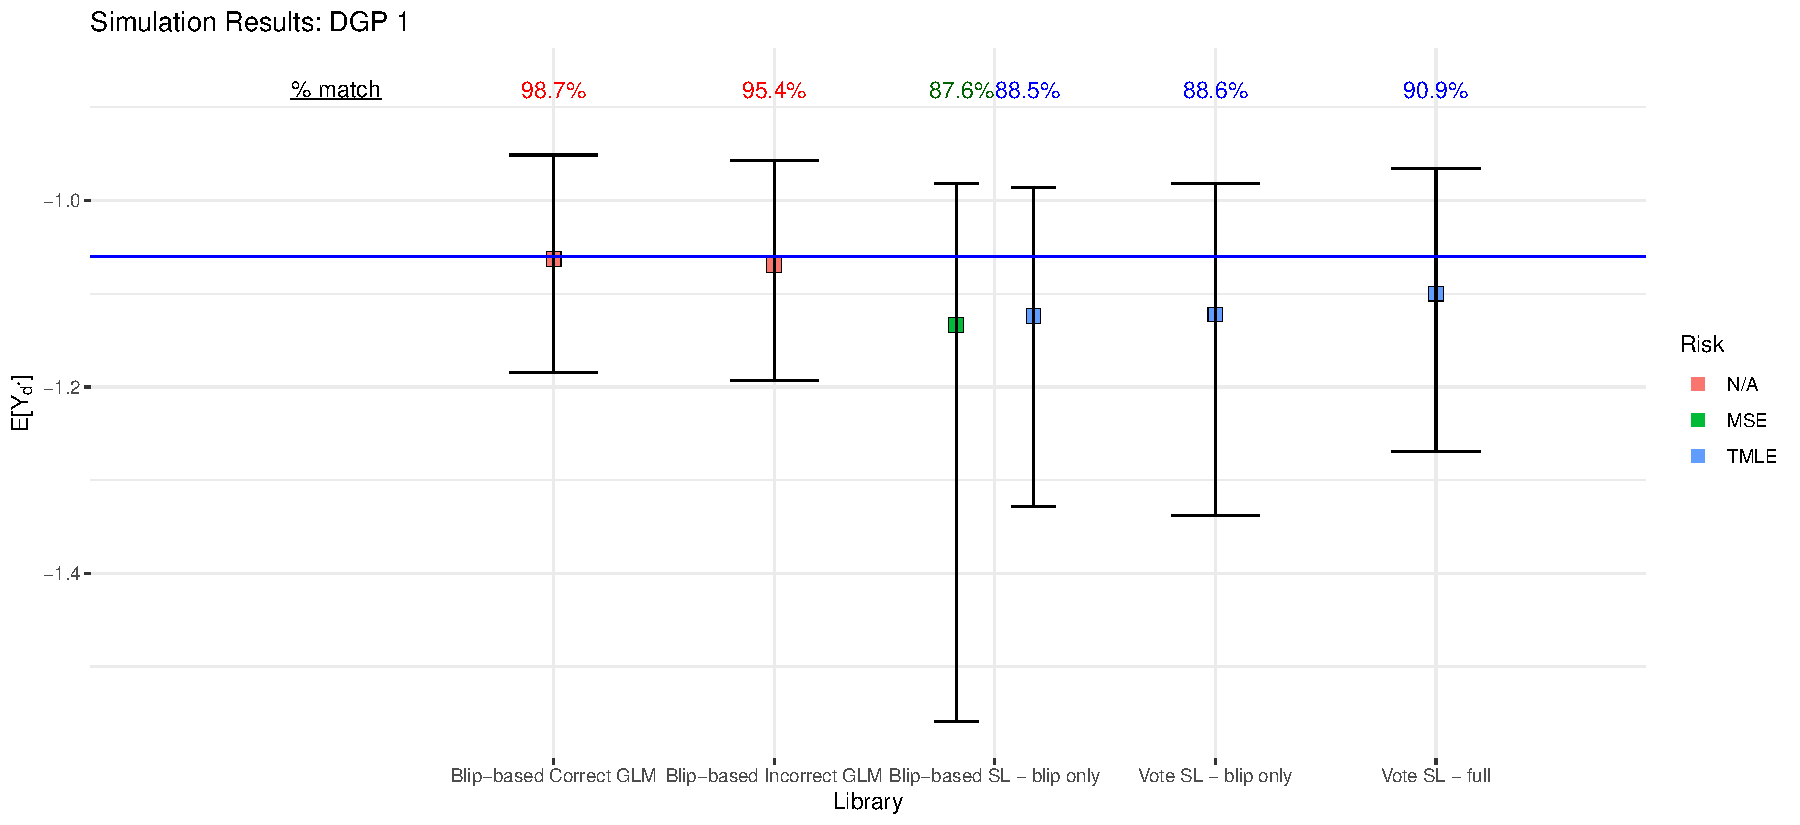
\includegraphics[width=\maxwidth]{figure/ODTR_DGP_smooth_step1a-1} 


% latex table generated in R 3.5.1 by xtable 1.8-4 package
% Sat Sep 14 17:01:30 2019
\begin{table}[ht]
\centering
\scalebox{0.7}{
\begin{tabular}{rrr}
  \hline
 & MSE & TMLE \\ 
  \hline
Bias & -0.07379 & -0.06421 \\ 
  Variance & 0.01443 & 0.00758 \\ 
  MSE & 0.01986 & 0.01170 \\ 
  coef.SL.glm & 0.44603 & 0.27515 \\ 
  coef.SL.mean & 0.13043 & 0.11315 \\ 
  coef.SL.glm.interaction & 0.10093 & 0.13870 \\ 
  coef.SL.earth & 0.08642 & 0.12161 \\ 
  coef.SL.nnet & 0.09612 & 0.13762 \\ 
  coef.SL.svm & 0.05824 & 0.09139 \\ 
  coef.SL.rpart & 0.08183 & 0.12237 \\ 
   \hline
\end{tabular}
}
\caption{smooth - SL blip based} 
\end{table}
% latex table generated in R 3.5.1 by xtable 1.8-4 package
% Sat Sep 14 17:01:31 2019
\begin{table}[ht]
\centering
\scalebox{0.7}{
\begin{tabular}{rr}
  \hline
 & TMLE \\ 
  \hline
Bias & -0.04020 \\ 
  Variance & 0.00632 \\ 
  MSE & 0.00793 \\ 
  coef.DonV.DonV.SL.glm\_All & 0.06711 \\ 
  coef.DonV.DonV.SL.mean\_All & 0.05509 \\ 
  coef.DonV.DonV.SL.glm.interaction\_All & 0.06046 \\ 
  coef.DonV.DonV.SL.earth\_All & 0.07712 \\ 
  coef.DonV.DonV.SL.nnet\_All & 0.06372 \\ 
  coef.DonV.DonV.SL.svm\_All & 0.06169 \\ 
  coef.DonV.DonV.SL.rpart\_All & 0.08113 \\ 
  coef.Qlearn & 0.07307 \\ 
  coef.OWL & 0.07239 \\ 
  coef.EARL & 0.10323 \\ 
  coef.optclass & 0.07881 \\ 
  coef.RWL & 0.06771 \\ 
  coef.treatall & 0.07068 \\ 
  coef.treatnone & 0.06779 \\ 
   \hline
\end{tabular}
}
\caption{smooth - SL vote all} 
\end{table}
% latex table generated in R 3.5.1 by xtable 1.8-4 package
% Sat Sep 14 17:01:31 2019
\begin{table}[ht]
\centering
\scalebox{0.7}{
\begin{tabular}{rr}
  \hline
 & TMLE \\ 
  \hline
Bias & -0.06252 \\ 
  Variance & 0.00854 \\ 
  MSE & 0.01244 \\ 
  coef.DonV.DonV.SL.glm\_All & 0.19664 \\ 
  coef.DonV.DonV.SL.mean\_All & 0.09887 \\ 
  coef.DonV.DonV.SL.glm.interaction\_All & 0.12916 \\ 
  coef.DonV.DonV.SL.earth\_All & 0.14071 \\ 
  coef.DonV.DonV.SL.nnet\_All & 0.14820 \\ 
  coef.DonV.DonV.SL.svm\_All & 0.11114 \\ 
  coef.DonV.DonV.SL.rpart\_All & 0.17527 \\ 
   \hline
\end{tabular}
}
\caption{smooth - SL vote blip} 
\end{table}
% latex table generated in R 3.5.1 by xtable 1.8-4 package
% Sat Sep 14 17:01:31 2019
\begin{table}[ht]
\centering
\scalebox{0.7}{
\begin{tabular}{rr}
  \hline
 & TMLE \\ 
  \hline
Bias & -0.00279 \\ 
  Variance & 0.00339 \\ 
  MSE & 0.00339 \\ 
  estimates..1.....grep.colnames.estimates..1.....pattern....coef... & 1.00000 \\ 
   \hline
\end{tabular}
}
\caption{smooth - correct blip GLM} 
\end{table}
% latex table generated in R 3.5.1 by xtable 1.8-4 package
% Sat Sep 14 17:01:31 2019
\begin{table}[ht]
\centering
\scalebox{0.7}{
\begin{tabular}{rr}
  \hline
 & TMLE \\ 
  \hline
Bias & -0.00944 \\ 
  Variance & 0.00344 \\ 
  MSE & 0.00352 \\ 
  estimates..1.....grep.colnames.estimates..1.....pattern....coef... & 1.00000 \\ 
   \hline
\end{tabular}
}
\caption{smooth - incorrect blip GLM} 
\end{table}








\end{document}
